%29/09 - Blanca
\chapter{Registro de imágenes}
El registro de imágenes hace referencia a alinear en un mismo sistema de coordenadas unas imágenes. Esto tiene varias aplicaciones. Si en un mismo sujeto adquieres varios tipos de imagen en distintos puntos temporales, se puede alinear para ver la evolución temporal de esa zona. También se puede hacer entre sujetos para automatizar un estudio. Además, cada tipo de imagen médica (TAC, PET) puede proporcionar una información distinta, por lo que al alinearlo se puede tener una visión más completa. Por todo esto, el proceso de alinear imágenes es diferente en función de lo que se quiera conseguir. Así, los tipos de abordajes de registro depende de lo que se busque. En general, se busca minimizar la diferencia entre la imagen de entrada y la salida, o maximizando la similitud. 

\section{Tipos de registro}
Hay distintos tipos de registro:
\begin{itemize}
\item \textbf{Registro rígido}: El registro rígido solo permite rotar, manteniendo distancias y ángulos, y mover en el plano.
\item \textbf{Registro de similaridad}: Se añade un multiplicador de escala. Puede rotar, mover y ampliar. Esta transformación escala todas las direcciones en la misma medida, conserva los ángulos y las proporciones relativas, e incluye rotación y traslación.
\item \textbf{Transformación afín:} Además de todo lo anterior, permite el shearing, que es la alteración de la imagen al modificar un solo eje. Mientras que el escalado mantiene la forma, el shearing no. No es uniforme, ya que puede tener distintas escalas en cada eje.

\begin{figure}[h]
\centering
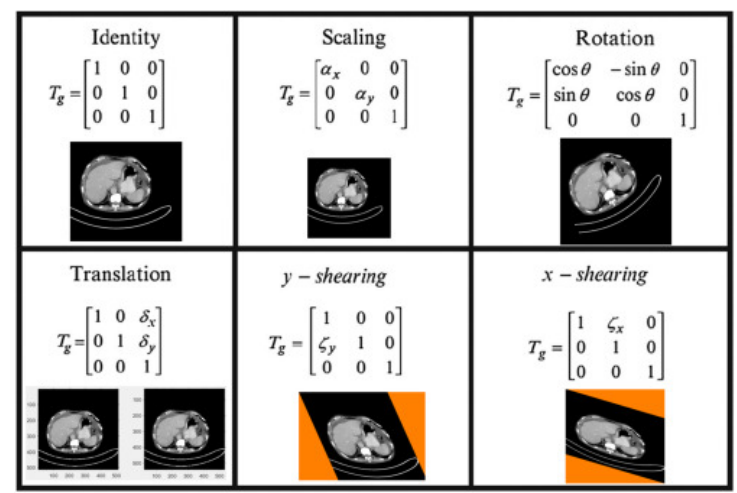
\includegraphics[width = 0.7\textwidth]{figs/registration.png}
\end{figure}

\item \textbf{Registro deformable:} Permite deformaciones locales que puede ser distinto para cada píxel. 
\item \textbf{Registro longitudinal:} Alinea múltiples imágenes del mismo sujeto a lo largo del tiempo, y puede seguir un registro rígido o deformable dependiendo de si se deben detectar cambios sutiles sin introducir deformaciones artificiales.
\item \textbf{Registro multimodal:} Alinea imágenes obtenidas mediante diferentes técnicas de imagen, como la resonancia magnética (estructural) y la tomografía por emisión de positrones (funcional). Las diferentes modalidades pueden tener contrastes distintos; entre las métricas de similitud comunes se incluyen la información mutua y la correlación cruzada. El registro multimodal preciso es fundamental para fusionar la información anatómica y molecular (por ejemplo, planificación quirúrgica, localización de tumores).
\end{itemize}

\begin{figure}[h]
\centering
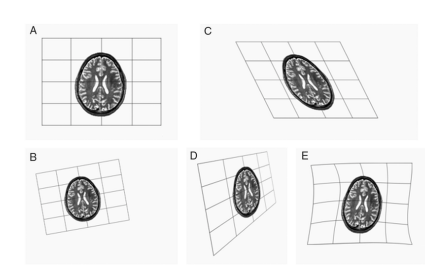
\includegraphics[width = 0.7\textwidth]{figs/registration-medical.png}
\caption{Un registro de imágenes médicas utilizando diferentes matrices de transformación. A) Una imagen original. B) Transformación de rotación y traslación. C) Transformación de rotación, traslación y cizallamiento. D) Transformación proyectiva. E) Transformación deformable.}
\end{figure}

\section{Avances clave en IA en registro de imágenes}
La IA está mejorando significativamente el registro y el co-registro de imágenes médicas al hacer que el proceso sea más rápido, más preciso y más robusto en entornos clínicos y de investigación.

Los modelos de aprendizaje profundo, como las redes neuronales convolucionales (CNN) y los modelos basados en transformadores, han revolucionado el registro de imágenes al aprender directamente cómo alinear imágenes a partir de ejemplos, saltándose el complejo diseño manual de características y la optimización iterativa.

Las arquitecturas CNN, como U-Net, predicen campos de deformación densos que describen los desplazamientos espaciales píxel a píxel necesarios para alinear las imágenes de forma rápida y precisa.

Los modelos basados en transformadores aportan la capacidad de aprender relaciones globales y dependencias contextuales en toda la imagen, lo que mejora la precisión del registro, especialmente en el caso de variaciones anatómicas grandes o complejas.

Los modelos de IA pueden realizar registros rígidos (traslación, rotación) y deformables (deformación no lineal), lo que ayuda a alinear órganos o tejidos que pueden haber cambiado de forma entre exploraciones.
 
A diferencia de los métodos de registro clásicos que se basan en procesos iterativos y métricas elaboradas manualmente, los algoritmos de IA realizan predicciones en un solo paso, lo que acelera enormemente el proceso de alineación y lo hace escalable para los flujos de trabajo clínicos.

Los enfoques de registro de IA se generalizan mejor en imágenes multimodales (por ejemplo, de PET a MRI) utilizando funciones de similitud aprendidas, superando las limitaciones de las métricas tradicionales basadas en la intensidad que tienen dificultades con los diferentes contrastes de las imágenes.

Estos avances permiten aplicaciones como la monitorización de la progresión de enfermedades, la planificación de tratamientos y estudios de investigación que requieren una alineación espacial precisa de grandes conjuntos de datos de imágenes.

\section{Artículo}
\textbf{Evaluación de un procedimiento de registro conjunto de imágenes multimodales (TC, RM y PET) en fantomas y pacientes con cáncer de cabeza y cuello: precisión, reproducibilidad y consistencia}

En el artículo busca mejorar la radioterapia en tumores. Se realiza una radiografía para ver el tumor y poder crear una terapia dirigida. Hay que tener en cuenta la intensidad de la radiación y la geometría del haz y dónde va a impactar en la anatomía del tumor. Para ello, se validan unas técnicas de corregistro entre distintas imágenes para delimitar lo mejor posible el volumen tumoral. Es un trabajo multi-técnica al utilizar PET (tomografía por emisión de positrones), TAC y resonancia magnética. Esto lo prueban en un phantom (tejido simulado para probar la técnica) y en pacientes. 

El objetivo del estudio era validar un método interactivo de corregistro rígido basado en segmentación de superficies para fusionar imágenes de CT, MRI y PET. Como sujetos se utilizaron fantomas diseñados con estructuras que simulan el cuello y 4 pacientes con carcinoma de células escamosas faríngeo-laríngeo.

Como referencia se utilizaba la tomografía computerizada (CT). Un observador ajustaba manualmente la traslación y rotación de una imagen sobre dicha referencia hasta lograr una superposición visual óptima. Los parámetros de transformación se guardaban.

El accuracy se definió como la diferencia entre la transformación aplicada por un observador y el valor promedio de todas las transformaciones realizadas por todos los observadores para la misma modalidad de imagen.
Se expresó como 2 desviaciones estándar de la distribución de las traslaciones y rotaciones. También se usó el vector euclidiano para combinar traslaciones en x, y, z y obtener un desplazamiento total en mm.

Se utilizó la reproducibilidad para medir cuán consistentes son los resultados cuando el mismo proceso lo realiza diferente gente o la misma persona en diferentes momentos. Se calculó la variación intra-observación (varianza de los resultados de corregistración de una misma persona 4 veces con días de separación) y variación inter-observador (4 observadores diferentes).  Se comparó esta varianza con la Varianza Residual (la varianza total que no se puede explicar por el observador), para ver si el factor "observador" era significativo.
Las variaciones intra e inter-observador fueron muy pequeñas (varianzas < 0.25 mm2) y muy inferiores a la varianza residual. Esto significa que el factor "observador" es insignificante y que cualquier clínico entrenado puede obtener resultados similares.

Finalmente, la consistencia medía si el método produce resultados coherentes cuando se aplica a diferentes tipos de imágenes del mismo sujeto. Para ello, se compararon los parámetros de coregistro obtenidos para las secuencias MRI T1 y MRI T2 de un mismo paciente. Como ambas se adquieren en el mismo equipo sin mover al paciente, deberían coregistrarse con los mismos parámetros. Cualquier diferencia indica una inconsistencia del método.
No hubo diferencias significativas al coregistrar MRI T1 vs. T2, excepto en una dirección (y), lo que sugiere que el método es robusto frente a cambios en el contraste de la imagen.

%Algunas imágenes son más anatómicas y otras más funcionales. Por ello, se distinguen imágenes de mapas. Los mapas se construyen a partir de varias imágenes. Las imágenes de difusión se utilizan mucho en clínica para procesos isquémicos en el cerebro. Mediante el movimiento de las moléculas de agua se puede ver el gradiente de los campos magnéticos para ver la estructura. Según la señal de resonancia magnética y las imágenes, se obtiene el valor de difusión a través de una fórmula matemática. Esto se registra y se construye un template. Los mapas se alinean con el template, el cual se debe bajar de resolución. 

\section{Imágenes, mapas y templates}
En el procesamiento de imágenes biomédicas conviene establecer una clara diferenciación entre lo que constituye una \textbf{imagen} y lo que representa un \textbf{mapa}. Las imágenes corresponden a datos directos adquiridos por los equipos de imagenología, como tomografías computarizadas, resonancias magnéticas o estudios de tomografía por emisión de positrones. Estos datos pueden presentarse en forma cruda o reconstruida, conteniendo información anatómica o funcional directa del paciente.

Por otro lado, los mapas representan datos derivados obtenidos mediante procesamiento matemático avanzado. Se construyen a partir de múltiples imágenes y encapsulan parámetros fisiológicos o físicos cuantitativos, proporcionando una representación numérica de propiedades tisulares específicas que no son directamente observables en las imágenes originales.

\subsection{Imágenes de Difusión en Neuroimagen}
Las imágenes de difusión por resonancia magnética se fundamentan en el movimiento browniano de las moléculas de agua en los tejidos biológicos. Desde la perspectiva física, esta técnica emplea gradientes de campo magnético específicamente diseñados para sensar el desplazamiento molecular. El movimiento de las moléculas de agua modula la señal de resonancia magnética de manera característica, permitiendo cuantificar las restricciones a la difusión mediante la atenuación de la señal observada.

En la práctica clínica, las imágenes de difusión han demostrado un valor incalculable para la detección de isquemia cerebral aguda. Durante un evento isquémico, se produce una restricción significativa de la difusión molecular que se manifiesta como una hiperintensidad característica en las imágenes ponderadas por difusión. Esta propiedad convierte a esta modalidad de imagen en una herramienta esencial para el diagnóstico temprano de accidentes cerebrovasculares, permitiendo intervenciones terapéuticas oportunas.

\subsection{Construcción de Mapas de Difusión}
La transición desde imágenes de difusión hacia mapas paramétricos implica un proceso de reconstrucción matemática sofisticado. El mapa de Coeficiente de Difusión Aparente (ADC) se obtiene mediante un ajuste por mínimos cuadrados realizado voxel por voxel, aplicando el modelo exponencial $S(b) = S(0) \cdot \exp(-b \cdot ADC)$, donde $S(b)$ representa la intensidad de señal con el gradiente de difusión aplicado, $S(0)$ denota la intensidad de señal sin gradiente de difusión, $b$ corresponde al factor de difusión expresado en $s/mm^2$ y $ADC$ simboliz el coeficiente de difusión aparente en $mm^2/s$.

El flujo de procesamiento comienza con la adquisición de múltiples imágenes de difusión utilizando diferentes valores del factor b. Posteriormente, se ejecuta la reconstrucción paramétrica mediante ajuste exponencial para generar el mapa de ADC voxel por voxel. La fase final incluye la validación y control de calidad del mapa resultante, asegurando la confiabilidad de las mediciones cuantitativas obtenidas.

\subsection{Registro de imágenes y templates}
En el contexto del análisis espacial estandarizado, los templates representan imágenes de referencia que definen espacios coordenados normalizados, como los sistemas MNI o Talairach. Estos templates poseen resoluciones espaciales predefinidas, típicamente de $1mm^3$ o $2mm^3$, y sirven como base fundamental para análisis multi-sujeto y comparaciones poblacionales.

El proceso de registro espacial implica la alineación geométrica de imágenes individuales con el template de referencia. Desde una perspectiva práctica, es la imagen individual la que normalmente se somete a re-muestreo para emparejar la resolución del template, estrategia conocida como \emph{downsampling}. Esta aproximación se justifica por el hecho de que los algoritmos de registro funcionan de manera óptima cuando las imágenes involucradas presentan resoluciones espaciales similares. Cabe destacar que en situaciones excepcionales donde el template presenta mayor resolución que la imagen individual, podría aplicarse el proceso inverso de \emph{upsampling}.